\section{Chapter 2 - Company Overview}
\subsection{About W3 Elites}

W3 Elites is a distinguished private enterprise, operating as a wholly-owned subsidiary of the renowned W3 Group. Established as a vanguard in recruitment consulting, W3 Elites plays a pivotal role in bridging the gap between talent and organizational needs. With a focus on aligning skilled professionals with roles that best suit their capabilities, W3 Elites assists its clients in realizing their full potential by ensuring that they are equipped with a workforce that is both efficient and strategically aligned with their business objectives.

As a premier provider of recruitment consultancy services in India, W3 Elites offers comprehensive, end-to-end recruitment solutions. Whether clients are in need of new talent or candidates are seeking employment opportunities, W3 Elites is dedicated to facilitating these connections with precision and expertise. The company’s mission is to match the right candidates to the right roles, delivering a tailored service that meets the unique demands of each client. W3 Elites’ extensive network and deep understanding of the industries it serves allow the company to provide career options across a wide spectrum of skills, including science, engineering, technical, and commercial domains. The consultants at W3 Elites are specialists in their fields, ensuring that clients receive the most informed and effective solutions possible.

In addition to traditional recruitment, W3 Elites offers a holistic array of services that includes Recruitment Process Outsourcing (RPO), staffing solutions, and startup scaling, particularly within the realms of IT, Human Resources, Sales, and Marketing. This comprehensive approach ensures that W3 Elites can address the full spectrum of recruitment needs, from initial talent acquisition to the scaling of new business ventures.

\begin{figure}[ht]
    \centering
    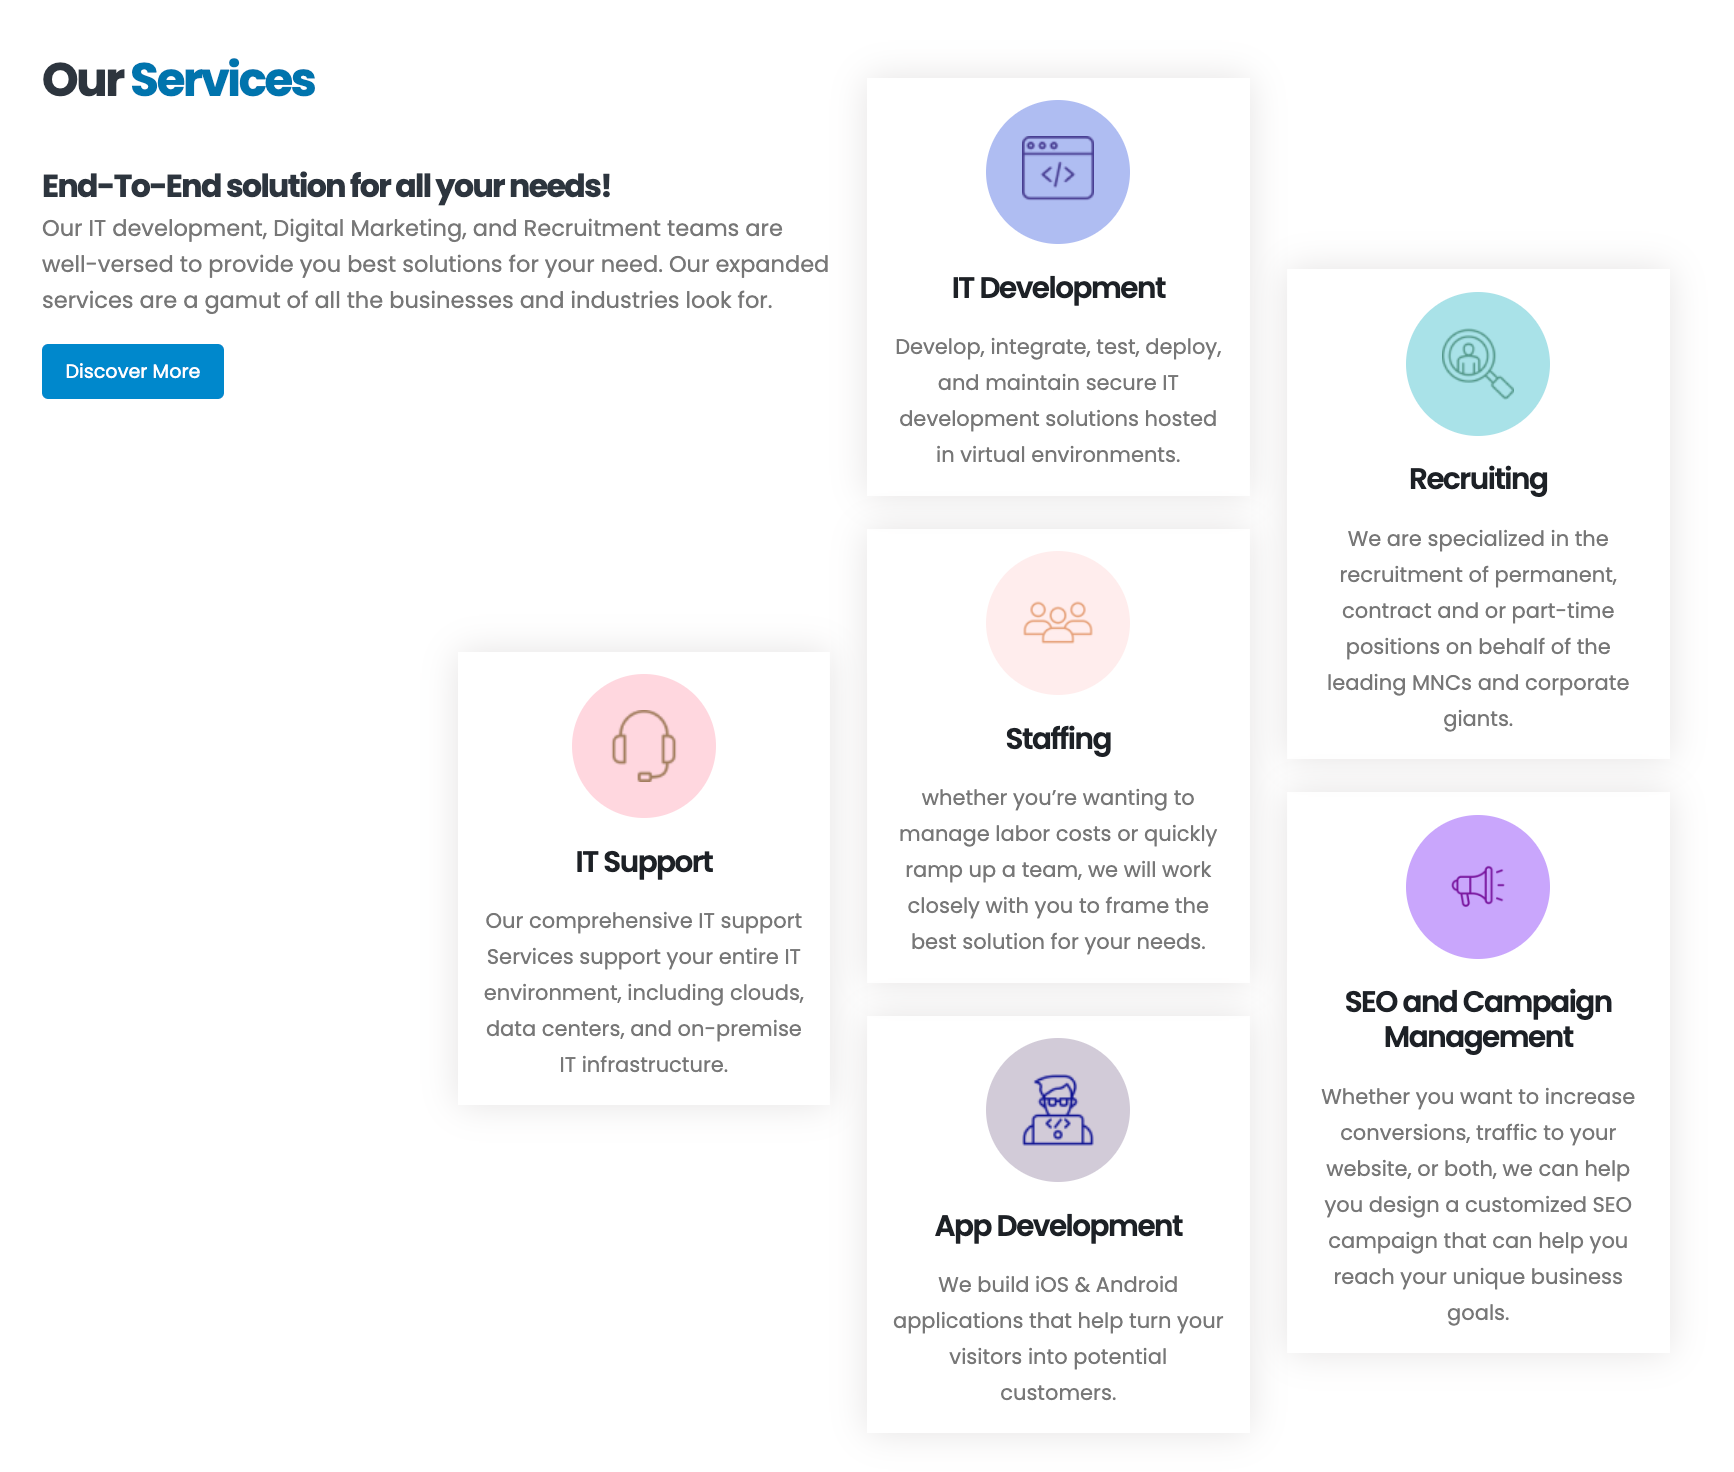
\includegraphics[width=0.1cm]{assets/w3elites-end-to-end.png}
    \caption{Flowchart illustrating the end-to-end recruitment process offered by W3 Elites.}
    \label{fig:recruitment_process}
\end{figure}

\subsection{Services and Products}

W3 Elites offers a broad range of services designed to meet the diverse needs of its clients. The core offerings include:

\begin{table}[h]
    \centering
    \caption{Comparison of Core Services Offered by W3 Elites}
    \begin{tabular}{|c|c|c|c|}
        \hline
        \textbf{Service} & \textbf{Benefits} & \textbf{Target Industries} & \textbf{Client Needs Addressed} \\
        \hline
        Recruitment Consulting & Strategic Workforce Enhancement & Multiple & Customized Recruitment Solutions \\
        \hline
        Staffing Solutions & Flexibility in Workforce Management & Dynamic Industries & Temporary/Permanent Staffing \\
        \hline
        RPO & Comprehensive Recruitment Management & Large Enterprises & End-to-End Recruitment Outsourcing \\
        \hline
        Startup Scaling & Rapid Business Growth Support & Startups & Talent Acquisition and Strategic Guidance \\
        \hline
    \end{tabular}
    \label{tab:core_services}
\end{table}

\begin{itemize}
    \item \textbf{Recruitment Consulting}: As a leader in the recruitment consulting sector, W3 Elites provides strategic advice and support to organizations seeking to enhance their workforce. The company’s consultants work closely with clients to understand their specific needs and provide tailored solutions that align with their business goals.
    \item \textbf{Staffing Solutions}: W3 Elites offers both temporary and permanent staffing solutions, enabling companies to scale their workforce up or down as needed. This flexibility is particularly valuable in industries with fluctuating demands, allowing clients to maintain optimal staffing levels without the burden of long-term commitments.
    \item \textbf{Recruitment Process Outsourcing (RPO)}: For organizations looking to outsource their entire recruitment process, W3 Elites offers a comprehensive RPO service. This includes everything from job posting and candidate screening to onboarding and post-placement support, allowing clients to focus on their core business activities.
    \item \textbf{Startup Scaling}: W3 Elites also specializes in helping startups scale their operations. By providing access to top talent and offering strategic guidance, the company helps startups grow quickly and efficiently, ensuring they have the human resources they need to succeed.

    
\end{itemize}



\subsection{The Team and Work Environment}

The team at W3 Elites is composed of highly skilled professionals who are not only experts in their respective fields but also deeply committed to the success of their clients. The work environment at W3 Elites is characterized by a culture of collaboration, innovation, and continuous learning. The company values diversity and fosters an inclusive workplace where every team member is encouraged to contribute their ideas and perspectives.

\textbf{Piyush Khandelwal}, the mentor for the internship program at W3 Elites, exemplifies the leadership qualities that define the company. As a Director at W3 Grads and a former mentor at GeeksforGeeks, Piyush brings a wealth of experience in software engineering, project management, and team leadership. His approach to mentorship is rooted in a deep commitment to developing the skills and careers of his team members, ensuring that they are well-prepared to tackle complex challenges and drive business results.

Piyush’s background in software engineering provides him with a strong foundation in problem-solving, which he has leveraged to successfully deliver numerous projects on time and within budget. His leadership style is both pragmatic and inspirational, combining strategic vision with hands-on guidance. Piyush is passionate about using his skills and experience to drive positive change, making a meaningful impact both within the company and in the broader industry.

\begin{figure}[h]
    \centering
    
\includegraphics[width=0.2cm]{assets/piyush.png}
    \caption{Portrait of Piyush Khandelwal, Director at W3 Elites.}
    \label{fig:piyush_khandelwal}
\end{figure}